\section{Sub Sections, Figures and Tables}~\label{sec:subsections}

In this chapter, how to the subsections and also the tables and figures are discussed in detail.

\subsection{Sub Section}\label{sec:subsection}
An example table is shown in Table~\ref{tab:dataset}.

\begin{table}[!ht]
\center
\caption{An example table.}
\label{tab:dataset}
\begin{tabular}{lccc}
\hline
Dataset Name& Classes & Training Set & Testing Set\\ \hline
Yelp P& $2$ & $560,000$ & $38,000$ \\
Yelp F& $5$ & $650,000$ & $50,000$ \\ 
Yahoo& $10$ & $1,400,000$ & $60,000$ \\  
Amazon F & $5$ & $3,000,000$& $650,000$ \\
Amazon P & $2$ & $3,6000,000$ & $400,000$ \\
DBPedia& $14$ & $560,000$ & $70,000$  \\
\hline
\end{tabular}
\end{table}


\subsubsection{Sub Sub Section}\label{sec:subsubsection}

An example figure is shown in Figure~\ref{fig:dataset}.

\begin{figure}[ht!]
    \centering
    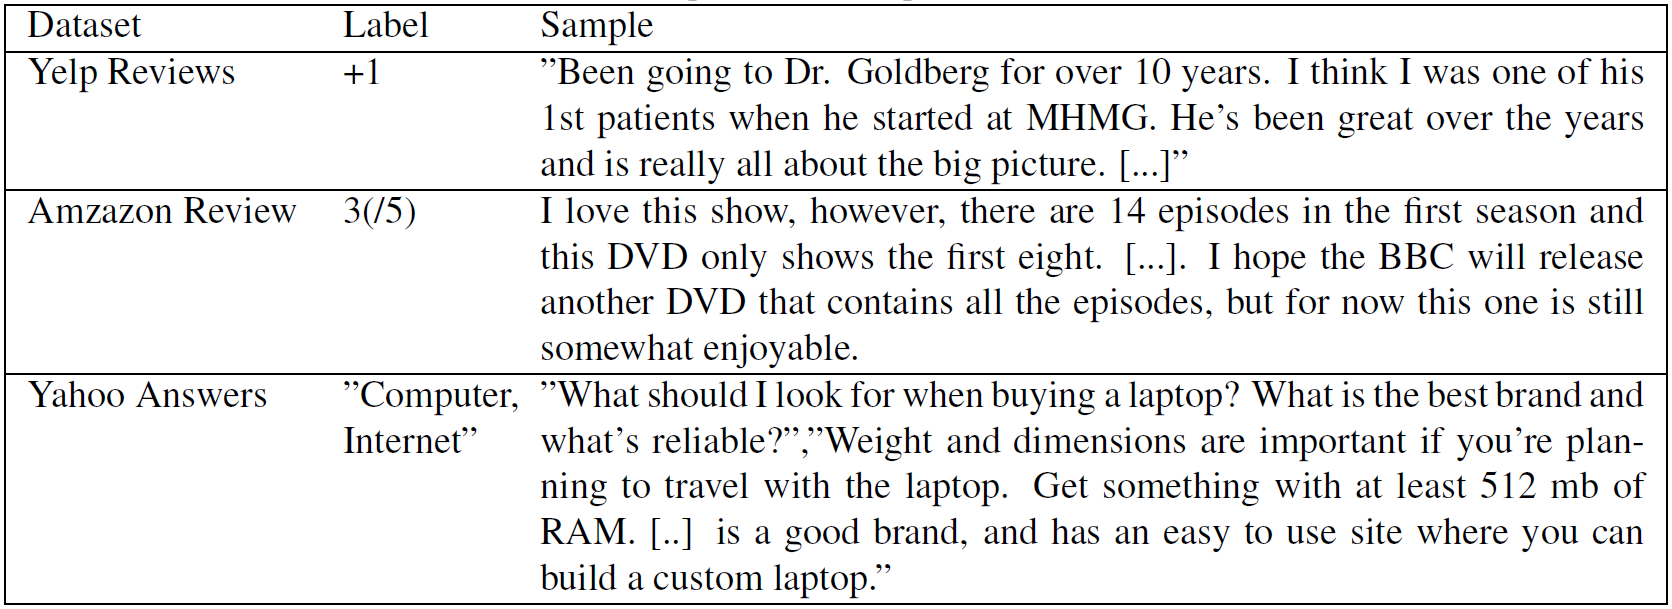
\includegraphics[width=1\columnwidth]{figures/dataset.png}
    \caption{An example figure.}
    \label{fig:dataset}
    \vspace{-3mm}
\end{figure}

 
\paragraph{Sub Sub Sub Section}\label{sec:subsubsubsection}
This is a Sub Sub Sub Section. This will not show up in the table of contents (TOC). If you want it to be shown, then set the ``tocdepth'' to 4 or more in thesis.tex.

\subparagraph{Sub Sub Sub Sub Section}\label{sec:subsubsubsubsection}
This is a Sub Sub Sub Sub Section. This will not show up in the TOC. If you want it to be shown, then set the ``tocdepth'' to 5 in thesis.tex.